\normaltrue
\correctionfalse

%\UPSTIidClasse{12} % 11 sup, 12 spé
%\newcommand{\UPSTIidClasse}{12}

\exer{Poutre encastrée $\star$ \label{C2:10:Def:531}}
\setcounter{question}{0}\UPSTIcompetence[2]{C2-10}
\index{Compétence C2-10}
\index{Torseur de cohésion}
\index{Déformée}


\footnotesize{D'après documents Emmanuel PINAULT-BIGEARD.}
\end{flushright}


\ifcorrection
\else
\marginnote{\textbf{Pas de corrigé pour cet exercice.}}
\fi

On donne la poutre suivante. 

\begin{figure}[H]
\centering
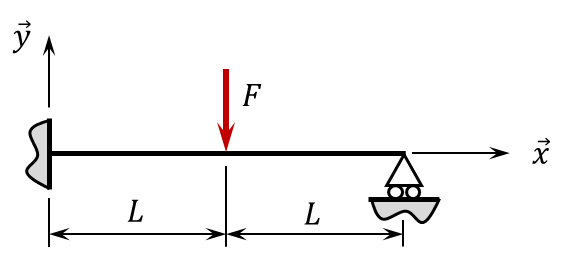
\includegraphics[width=\linewidth]{531}
%\caption{\label{61_01} Loi de commande de vitesse en trapèze}
\end{figure}

Données : 
\begin{itemize}
\item $\vect{F}=-F\vect{y}=-\SI{2000}{y}$;
\item Poutre IPE 80;
\item $I_{G_z} = \SI{801400}{mm^4}$;
\item $E = \SI{200000}{MPa}$;
\item $G = \SI{80000}{MPa}$;
\item $L= \SI{1}{m}$.
\end{itemize}

\question{Déterminer l'inconnue hyperstatique.}
\ifprof
\else
\fi

\question{Donner la valeur de la flèche au point d'application de l'effort.}
\ifprof
\else
\fi



\ifprof
\begin{figure}[H]
\centering
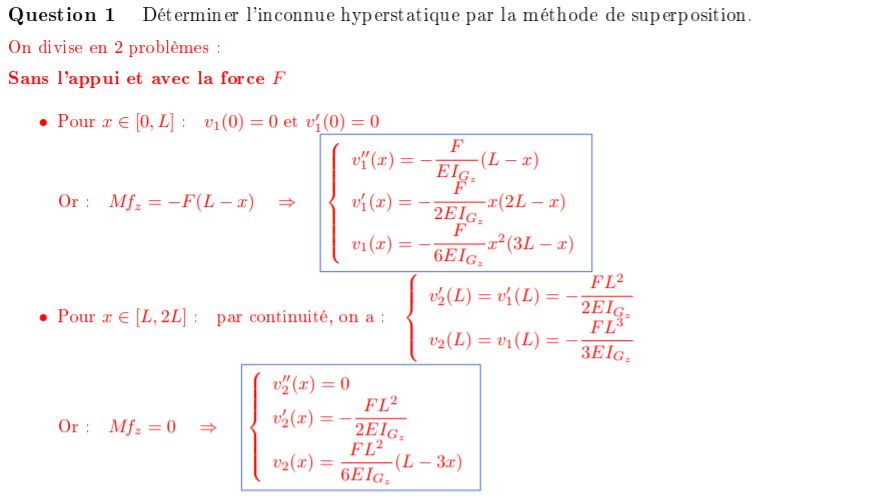
\includegraphics[width=\linewidth]{531_01_c}
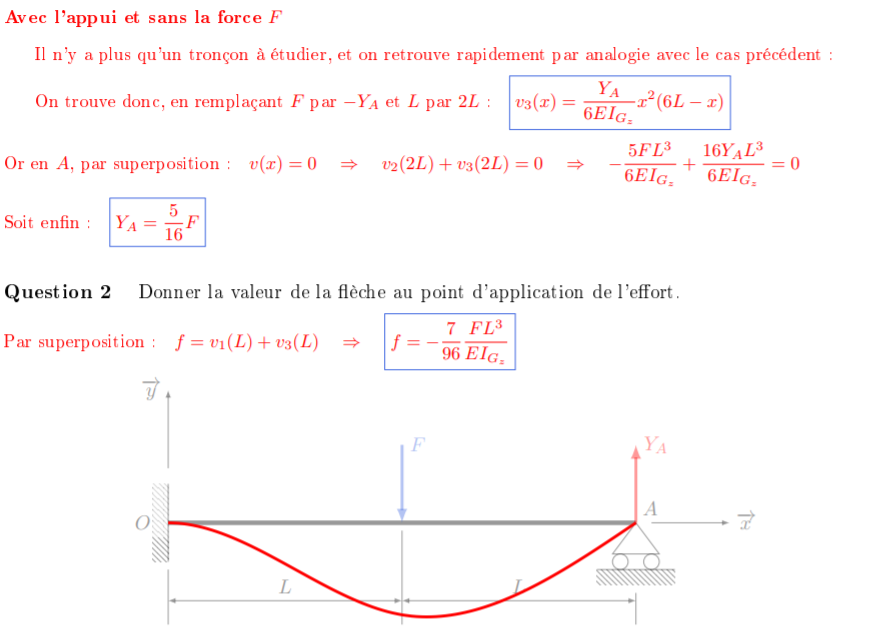
\includegraphics[width=\linewidth]{531_02_c}
\end{figure}
\else
%\footnotesize
%\begin{enumerate}
%  \item $\left(fp + Mp^2\right) Z(p)=S_h P_h(p)-S_e P_e(p) - \dfrac{Mg}{p}$
%    \item $Q_e(p)=\left(S_a - S_b \right)pL(p) + \dfrac{V_t}{B_e} p P_e(p)$ et $mp^2 L(p) = -rL(p)+\left(S_a-S_b\right) P_e(t)-f'pL(p)$.
%\end{enumerate}
%\normalsize


\marginnote{Corrigé voir \ref{C2:10:Def:531}.}

\fi